\chapter{数值程序优化方法}\label{chapter_framework}

在这一章节中,我们首先以一个具体的实例来阐释一下本文优化方法的基本思想,然后我们会对整个优化过程进行一个整体的介绍,整个优化过程一共包含了稳定性分析、路径提取、随机代数变换以及路径合并这四个不同的部分,本章剩余的部分则是对这四个不同的部分进行的具体介绍。

\section{方法简介}
在本小节中,我们举一个具体的例子来阐释整体的程序优化方法,此优化实例的计算程序来自于\cite{doi:10.1137/08074218X}。如图\ref{fig:midarc}所示,在复平面内有两个单位复数$z_1,z_2$,我们需要计算这两个负数在复平面上的角平分线所对应的单位复数$z_3$。依据一定的数学上的背景知识,当$z_1,z_2$均为单位复数时,计算$z_3$只需要通过以下公式进行计算:
\begin{gather*}\label{eq:fpex}
    z_3=\frac{z_1+z_2}{\left|z_1+z_2\right|}
\end{gather*}
软件开发人员根据以上公式,可以非常轻易地实现整个计算过程,代码如图\ref{lst:exoricode}所示。这样的代码非常符合人们的直观感受并且非常易读易维护,然而这样的代码并不是正确并且高效的代码。如果我们使用任意精度类型来实现这样的代码,程序的运行效率会比普通的浮点精度实现慢上成百上千倍。而如果我们使用浮点精度类型来实现这样的代码,后果更为严重,这样的程序甚至是错误的。通过的计算过程的简单分析我们可以知道,当我们使用浮点精度类型去实现这个计算过程时,如果$|z_1+z_2| < \epsilon$的话,其中$\epsilon$是一个很小的正数,整个计算过程将会是不稳定的。

\begin{figure*}[thbp]
   \centering
   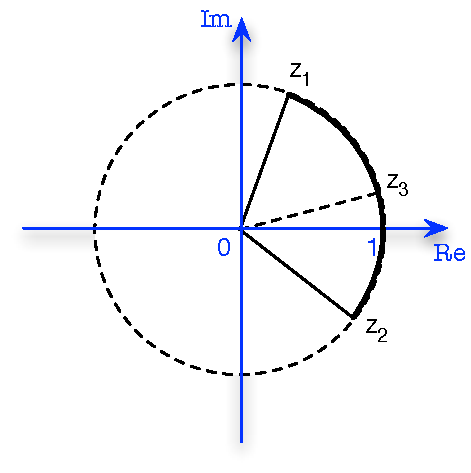
\includegraphics[width=88mm]{fig/ExampleArc_formal.pdf}
   \caption{单位复数复平面角平分线示意图} \label{fig:midarc}
\end{figure*}

当$|z_1+z_2| < \epsilon$时,在程序代码的第4行与第5行,计算$z_1+z_2$时,由于$z_1 \approx -z_2$,这个加法操作会产生相近数相减的情况\cite{NumericalAnalysis},使得计算结果的有效数字位数发生锐减,导致计算结果的相对误差非常大。而后续第7行的除法操作,由于除数$|z_1+z_2|$是一个非常小的数,会进一步放大前面加法操作的误差,导致程序的计算结果出错。我们实际运行了一下这个程序,在处理器为英特尔酷睿i7 2.9GHz的苹果笔记本MacBook Pro上,以浮点精度类型实现的该计算过程,我们令输入$z_1=e^{i\pi/4},z_2=-z_1*e^{-i \epsilon \pi},\epsilon=10^{-16}$,程序的运行结果$z_3=-0.5547+0.8321i$,显而易见是错误的,其正确结果应该为$z_3=-0.7071+0.7071i$。

\begin{figure}[thbp]
    \begin{lstlisting}[%
      xleftmargin=7em,numberblanklines=true,boxpos=b,%,extendedchars=\true, %inputencoding=utf8%/latin1
      morekeywords={REAL,IComplex}%keywords={main}
    ]
    IComplex midarc(IComplex z1,IComplex z2){
      if(abs(z1)!=1 || abs(z2)!=1)
        throw PreConditionException;
      REAL r = realpart(z1) + realpart(z2);   
      REAL i = imaginary(z1) + imaginary(z2); 
      IComplex sum(r,i);
      IComplex z3 = sum / abs(sum);           
      return z3;
    }
    \end{lstlisting}
    %\vspace*{-4mm}
    \caption{公式$(z_1+z_2)/|z_1+z_2|$计算$z_3$的任意精度代码}
    \label{lst:exoricode}
    %\vspace*{-4mm}
\end{figure}
    
我们的优化框架可以将图\ref{lst:exoricode}中这样的不稳定的浮点精度的计算过程优化成为稳定高效的浮点精度的计算过程,如图\ref{lst:exoptcode}所示。 原来不稳定的计算过程$z_3=(z_1+z_2)/|z_1+z_2|$被转换成了一种与之在数学上等价的稳定的计算过程,具体来说,$z_1,z_2,z_3$均被表示成了复数的极坐标表示形式,$z_1=e^{i\theta_1},z_2=e^{i\theta_2}$,与此同时,$z_3$的计算过程也被等价的转换成为:

\begin{gather*}\label{eq:optex}
    z_3=e^{\frac{\theta_1+\theta_2}{2}i}
\end{gather*}

当$|z_1+z_2|<\epsilon$时,优化后的代码便使用这样稳定的计算过程来计算$z_3$,这样一来,优化后的代码便避免了原本不稳定的计算操作。同样的,我们以输入z$z_1=e^{i\pi/4},z_2=-z_1*e^{-i \epsilon \pi},\epsilon=10^{-16}$来运行优化后的代码,得到的结果即为正确的运行结果$z_3=-0.7071+0.7071i$。

\begin{figure}[thbp]
  \begin{lstlisting}[%
    xleftmargin=5em,numberblanklines=true,boxpos=b,%,extendedchars=\true, %inputencoding=utf8%/latin1
    morekeywords={FComplex}%keywords={main}
  ]
  FComplex midarc(FComplex z1,FComplex z2){
    if((abs(z1)-1)>epsi || (abs(z2)-1)>epsi)
      throw PreConditionException;
    double r = realpart(z1) + realpart(z2);      
    double i = imaginary(z1) + imaginary(z2);    
    FComplex sum(r,i); FComplex z3;              
    if(abs(sum)<epsi){
      double theta1 = atan2(imaginary(z1),realpart(z1));
      double theta2 = atan2(imaginary(z2),realpart(z2));
      double theta3 = (theta1+theta2)/2;
      z3 = FComplex(cos(theta3),sin(theta3));
    }else{
      z3 = sum / abs(sum);                       
    }
    return z3;
  }
  \end{lstlisting}
  %\vspace*{-4mm}
  \caption{优化后示例程序代码}
  \label{lst:exoptcode}
  %\vspace*{-4mm}
\end{figure}

整个优化过程的主要思想是通过代数式的等价转化,将原本不稳定的浮点精度计算过程替换成为一个与之等价的稳定的计算过程,每次这样的计算过程的替换都必须保证替换前后的计算过程在数学意义上是等价的。这样的替换过程的主要难点在于如何自动地寻找这样一个等价的稳定计算过程,因此本文提出了一种基于随机代数变换的等价表达式搜索算法,将这样一个替换过程转变成为一个搜索的过程。首先,我们会将数值程序的计算过程作为一个整体抽取出来,得到一个计算过程的代数式(在上述例子中,这个代数式便是$z_3=(z_1+z_2)/|z_1+z_2|$),然后我们对该代数式进行随机的代数变换,变换过程如图\ref{fig:eqspace}所示,得到新的等价代数式后,我们会将其加入到等价代数式集合中去,接着我们会在整个等价集合中随机选取代数式然后继续进行随机的变换,这样迭代下去,一直到我们寻找到一个稳定的计算代数式。当我们找到了稳定的计算代数式后,我们会将这个代数式还原成为可执行代码,并替换原不稳定的计算过程。

\begin{figure}[thb]
  \centering
  \vspace*{1mm}
  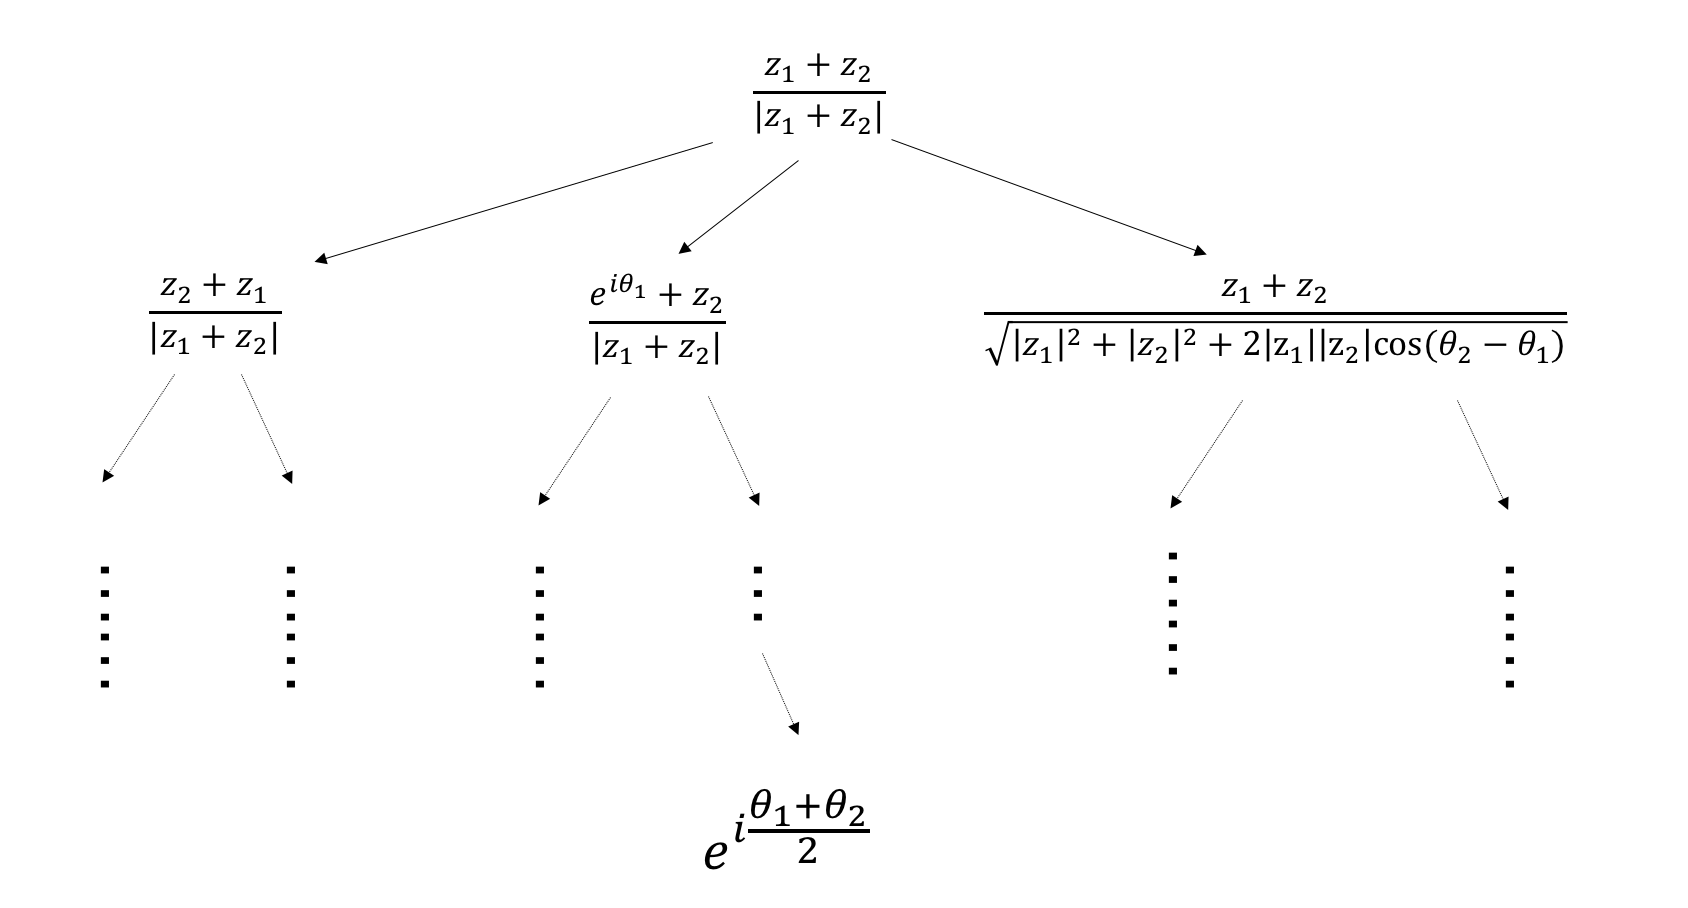
\includegraphics[width=\columnwidth]{fig/EquivalentSpace.png}
  \vspace*{1mm}
  \caption{等价代数式变换过程示意图} \label{fig:eqspace} %Equivalence Space to Find a Stable Algebraic Form
\end{figure}

\section{优化算法}
在上一小节中我们以一个具体的实例说明了整体的优化过程,在这一小节中,我们将会具体讨论优化方法的具体构成以及一些技术细节。如图\ref{fig:mainframe}所示,数值程序的优化过程一共分为4个模块,包括了稳定性分析模块、计算路径提取模块、随机代数变换模块以及计算路径合并模块。
首先,稳定性分析模块会使用区间分析的技术对原程序进行稳定性的分析,对程序的输入域进行划分,将程序的输入域划分为稳定区间,不稳定区间以及未知区间,这三种不同类型区间的具体含义会在下面具体介绍。紧接着,计算路径提取模块会通过符号执行的方式,将不稳定区间所对应的计算过程进行提取,得到程序输出关于程序输入的一个计算代数形式。然后,随机代数变换模块对上个模块提取到的计算代数式进行数学意义上的等价变换,寻找到原计算过程的等价的稳定的计算形式。最后,路径合并模块将上个模块中的等价稳定计算形式转换成为代码片段,并与原本就稳定的计算路径进行合并,得到最终的优化后程序。

\begin{figure*}[thbp]
  \centering
 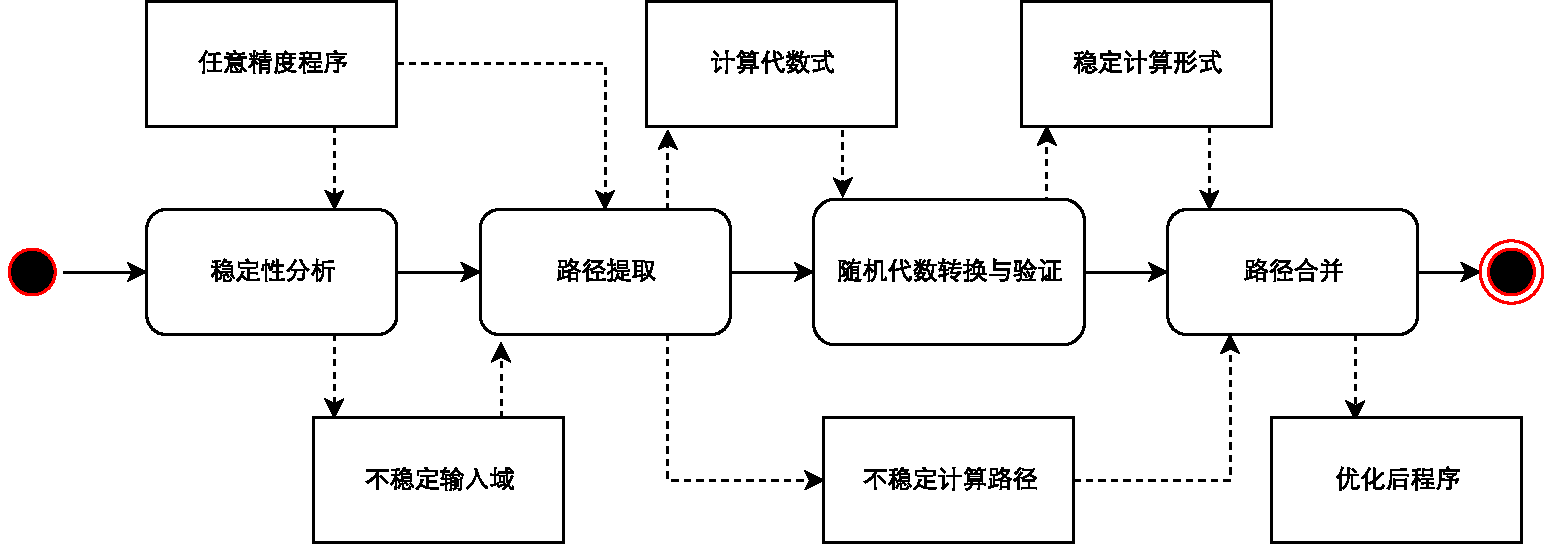
\includegraphics[width=\textwidth]{fig/MainFramework.pdf}
  \caption{数值程序优化框架整体流程图} \label{fig:mainframe}
\end{figure*}

\subsection{稳定性分析}

\subsubsection{稳定输入域定义}
对于一个计算过程$f$来说,我们记其浮点精度实现与任意精度实现所对应的计算过程分别为$F$和$M$,$D$为程序的输入域,对于任意输入$x \in D$,记$F(x)$与$M(x)$分别为以输入$x$去执行计算过程$f$的浮点精度实现以及任意精度实现所得到的计算结果。如果对一个输入域$I \subseteq D$,$I$上的任意输入$x$满足:
\begin{align*}
  \Big|\frac{F(x)-M(x)}{M(x)}\Big| < \varepsilon
\end{align*}

则我们称该输入域$I$为一个稳定的输入域。反之,若存在$x \in I$,使得:
\begin{align*}
  \Big|\frac{F(x)-M(x)}{M(x)}\Big| \geq \varepsilon
\end{align*}

则我们称该输入域为不稳定输入域,其中$\varepsilon$为参数,是一个很小的正数,用来表示优化过程中所能容忍的两种不同精度实现计算结果的最大的相对误差。

\subsubsection{输入域划分}

稳定性分析模块会将程序的输入域划分成为稳定输入域以及不稳定输入域,对于稳定输入域部分,由于其本身计算过程已经是稳定的,我们只需要将原计算过程直接使用浮点精度实现即可(对应图\ref{lst:exoptcode}中第13行),然而对于不稳定的输入域,其中包含了会产生误差的输入,优化框架需要对这样的输入域对应的计算过程进行优化(对应图\ref{lst:exoptcode}中第8行到第11行)。

如图\ref{fig:inputspace}为对数值计算程序输入域的一个整体的划分。理论上来讲,整个输入域可以完全的划分成为两个不相交的集合分别为稳定输入域以及不稳定输入域,然而这项工作在现实实践中是非常困难的。通过本节所介绍的分析技术,稳定性分析模块可以识别出部分的稳定输入域以及不稳定输入域,而剩余的无法识别的部分稳定性分析模块会将其归入未知输入域。在整个优化框架中,对于未知输入域以及无法找到稳定计算过程的不稳定输入域,我们会保留原始的任意精度计算过程以保证程序最终计算结果的正确性。

\begin{figure}[tb]
  \centering
  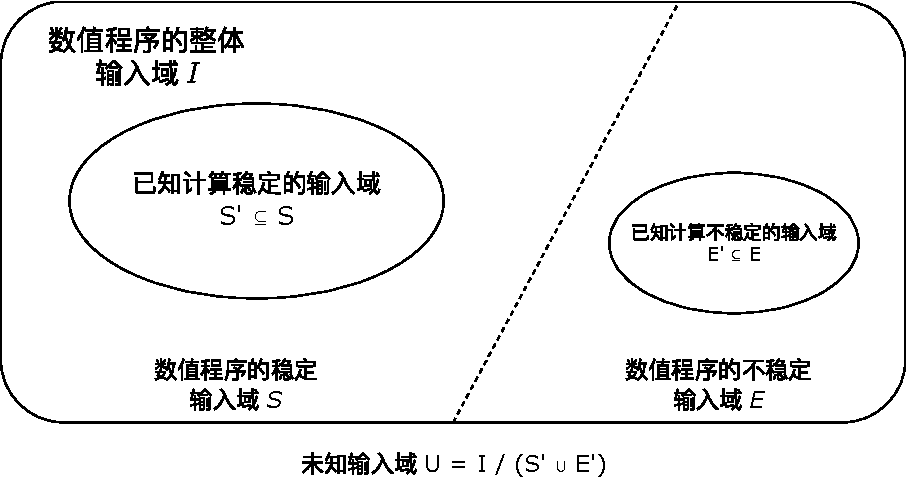
\includegraphics[width=\columnwidth]{fig/InputSpace.pdf}
  \vspace*{1mm}
  \caption{数值计算程序输入域划分图} \label{fig:inputspace} %Equivalence Space to Find a Stable Algebraic Form
\end{figure}

\subsubsection{稳定性分析整体算法}

稳定分析的整体算法流程如图\ref{alg:stabilityAnalysis}所示,我们首先会对程序的整体输入域进行划分,将其划分为多个小区间,然后对小区间进行稳定性的分析。这样做的原因如下:一方面对于一个较大的输入域,其可能即包含了一部分稳定的输入域,又包含了一部分不稳定的输入域,无法对其直接进行分类,然而,对于一个很小的输入域来讲,当其足够小时,其包含的输入较为有限,因此其稳定性也更加容易确定。另一方面,由于使用区间分析方法往往会高估其分析的结果,所以当输入域较小时其分析的结果也会更为准确。基于以上两点原因,在进行稳定性分析时,我们首先会将程序的输入域划分为许多小区间,然后我们对每个小区间的稳定性进行判定,然后再将相同类型的小区间合并起来得到最终的稳定输入域,不稳定输入域以及未知输入域。在算法\ref{alg:stabilityAnalysis}中,第1行对应的便是对整个的输入域进行划分,将其划分为多个等宽的小区间。接着,对每个小区间,我们会通过区间分析的技术判定该小区间上的最大误差是否在一个可以接受的范围内,如果是,我们便认为该小区间是稳定的,将其列入稳定的输入域,这一过程对应算法\ref{alg:stabilityAnalysis}中的第3-4行。由于区间分析技术有可能会放大该计算过程的最大误差,所以当我们的判定过程得到的最大误差超出可接受范围时,我们无法立即判定该小区间是不稳定的,这时候,我们会尝试去寻找该小区间中可能会引发不稳定计算的输入,具体的做法便是在该小区间内随机的取一些输入点,比较这些输入点在浮点精度计算以及任意精度计算下的计算结果,是否有较大偏差。如果发现产生了较大偏差,则判定该小区间是不稳定的,对应算法\ref{alg:stabilityAnalysis}中的第6-10行。也有可能的情况是,我们即无法使用区间分析的技术验证一个计算过程是稳定的,又无法在其中寻找到能够引发不稳定计算的输入点,对于这样的小区间,我们将其划分为未知输入域,即无法判定其稳定性的区间,对应算法\ref{alg:stabilityAnalysis}中的第12行。
\begin{algorithm}[thb]
  \caption{稳定性分析算法}
  \label{alg:stabilityAnalysis}
\begin{algorithmic}[1]
\REQUIRE $D$ {{\footnotesize$//$}\small 程序输入域}
\ENSURE $S', E', U$ {{\footnotesize$//$}\small 稳定性分析结果,包括了稳定输入域、不稳定输入域以及未知输入域}
\STATE $\{ d \}$ $\leftarrow$ split($D$) {{\footnotesize$//$}\small 将原程序的输入域划分为多个小区间}
\FORALL {$d_i \in \{ d \}$}
\IF {isIntervalStable($d_i$)}
\STATE add($d_i$, $S'$)
\ELSE
\STATE $\{ p \}$ $\leftarrow$ randomSamplePoints($d_i$) {{\footnotesize$//$}\small 在小区间$d_i$上随机采点}
\FORALL {$p_i \in \{ p \}$}
\IF{$\neg$ checkStable($p_i$)}
\STATE add($d_i$, $E'$)
\ENDIF
\ENDFOR
\STATE add($d_i$,$U$) {{\footnotesize$//$}\small 所有的采样点均计算稳定,无法判断该小区间的稳定性}
\ENDIF
\ENDFOR
\end{algorithmic}
\end{algorithm}

\subsubsection{小区间稳定性判别原理}

经过上述的论述们知道,对于一个小区间$I$来说,若对于任意$x \in I$,满足的$|\frac{F(x)-M(x)}{M(x)}| < \varepsilon$话,我们可以称该小区间是稳定的。也就是说,我们需要能够保证在该小区间上的任意输入在浮点精度下的计算结果与任意精度下的计算结果相差不是很大,在一个我们可以接受的范围内。在第二章相关工作中我们介绍了区间分析技术以及仿射算法,如果我们将计算过程P的浮点精度实现以及任意精度实现在经过区间分析得到的结果分别记为$F(I)$与$M(I)$,根据区间分析的定义我们可以得到:
\begin{align*}
  \max\Big\lbrace \frac{|F(x)-M(x)|}{|M(x)|} \, \Big| \, x \in I \Big\rbrace \subset \frac{|F(I) - M(I)|}{|M(I)|}
\end{align*}
因而我们可以得到:
\begin{align*}
  \max\Big\lbrace \frac{|F(x)-M(x)|}{|M(x)|} \, \Big| \, x \in I \Big\rbrace < \max \Big\lbrace x \, \Big| \, x \in \frac{|F(I) - M(I)|}{|M(I)|} \Big\rbrace
\end{align*}
因此对于一个小区间$I$来说,若其满足:
\begin{align*}
  \max \Big\lbrace x \, \Big| \, x \in \frac{|F(I) - M(I)|}{|M(I)|} \Big\rbrace < \varepsilon
\end{align*}
则我们可以认为该小区间是计算稳定的。

根据我们对不稳定输入域的定义,只要小区间$I$上存在一个输入使得计算过程$P$产生不稳定计算,则我们便认为该小区间I计算不稳定。因此,在判定一个小区间是否是不稳定时,我们只需要采用证否的方法,我们选择在该小区间内随机选取采样点,观察这些采样点在浮点精度下与任意精度下的相对误差是否超过了$\varepsilon$若找到了这样的点,我们则认为计算过程$P$在小区间$I$上是不稳定的,若没有找到,我们则将小区间$I$归入未知区间。

\subsection{路径提取}
为了对不稳定输入域上的计算过程进行优化,我们必须将这些计算过程作为一个整体从程序中提取出来,整个计算过程被抽象成为了程序输出关于程序输入的一个计算代数式的形式,这便是路径提取模块所要完成的工作。并且,对于不同输入域上的输入,其对应的计算过程有可能是不同的,对应到程序的控制流图上,即程序在不同输入域上在程序控制流图上所执行的路径时不同的,我们需要对不稳定输入域上涉及到的所有的程序执行路径进行提取。在对程序的执行路径进行提取的同时,路径提取模块同时还会收集每一条执行路径所对应的约束,以便于后续计算过程优化结束后组合程序时使用。原计算过程经过路径提取后被抽象成为了(路径约束,计算代数式)这样的二元组的集合的形式,集合中每个元素均为一个二元组,代表了程序控制流图中的一条执行路径,包含了该执行路径的计算代数式以及对应的约束信息。

下面举一个具体的实例来描述路径提取模块的执行结果,如图\ref{lst:symextexam}所示为计算$f(a,b)=|a|+|b|$的数值程序代码片段。其对应的程序控制流图如图\ref{fig:cfg}所示,此程序中总共包括了4条不同的执行路径,优化框架对其进行路径提取的结果如图\ref{fig:cfge}所示,路径提取会收集每条程序执行路径上的约束信息以及我们所关注的输出变量的计算表达式。在这个例子中,4条不同的执行路径分别对应着输入$a$,$b$取值为正或者为负的情况,每条路径提取得到的计算表达式也不同。

\begin{figure}[htbp]
  \centering
  \begin{minipage}[b]{0.58\textwidth}
  \centering
  \begin{lstlisting}[%
      xleftmargin=0em,numberblanklines=true,boxpos=b,%,extendedchars=\true, %inputencoding=utf8%/latin1
      morekeywords={REAL,IComplex}%keywords={main}
    ]
    double abs_sum(double a, double b) {
        double r = 0.0;
        if ( a > 0 ) { 
            r += a; 
        } else { 
            r -= a;
        }
        if ( b > 0 ) {
            r += b;
        } else {
            r -= b;
        }
        return r;
    }
  \end{lstlisting}
  \caption{计算$f(a,b)=|a|+|b|$代码片段}
  \label{lst:symextexam}
  \end{minipage}
  \begin{minipage}[b]{0.38\textwidth}
  \centering
  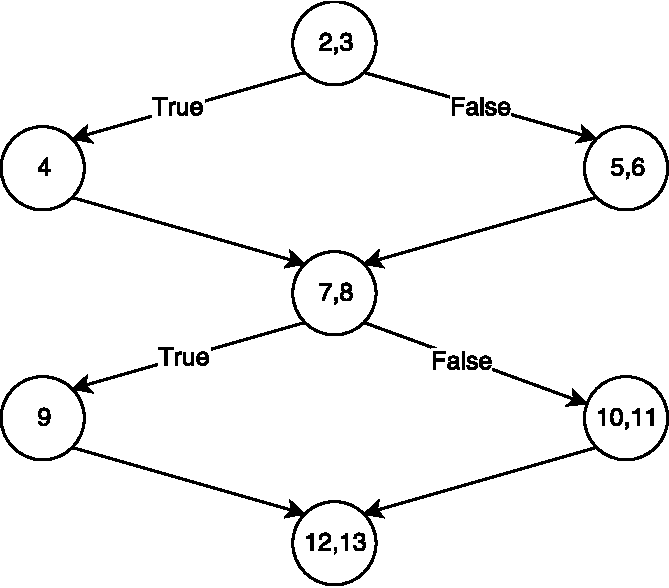
\includegraphics[width=6cm]{fig/ControlFlowGraph.pdf}
  \caption{程序$f=|a|+|b|$控制流图} \label{fig:cfg}
  \end{minipage}
\end{figure}
  

\begin{figure*}[thbp]
  \centering
  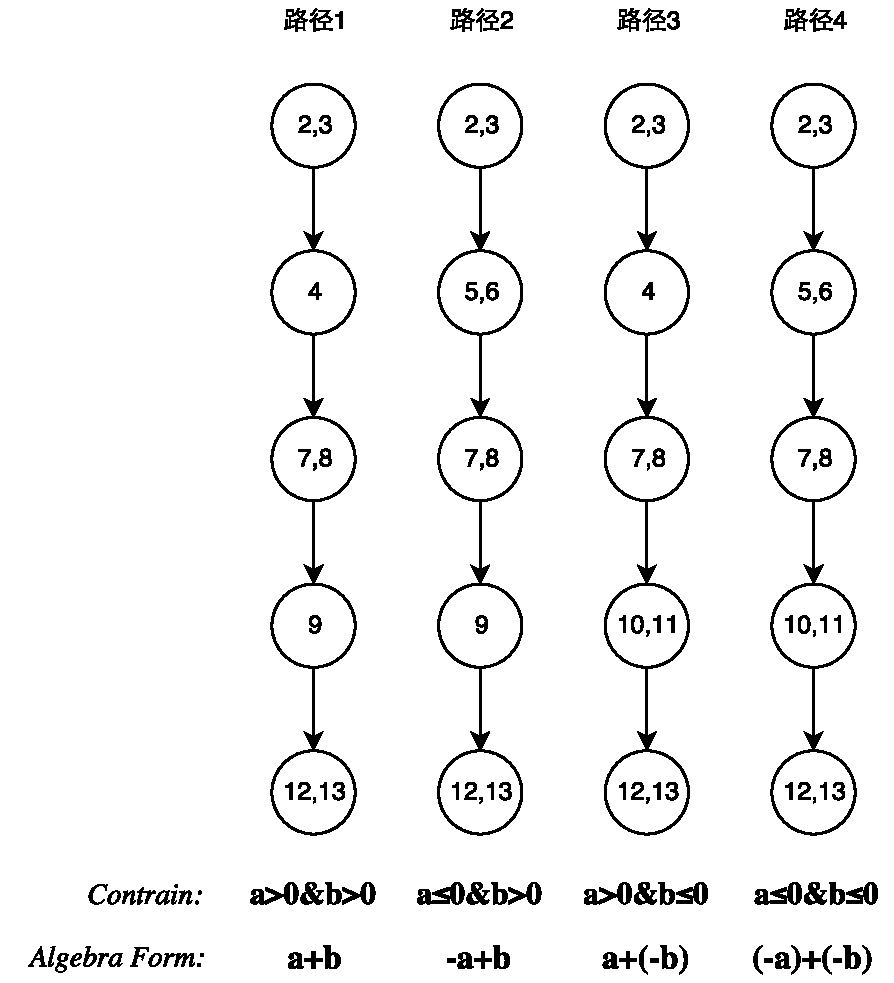
\includegraphics[width=110mm]{fig/ControlFlowGraphExtracted.pdf}
  \caption{程序$f=|a|+|b|$路径提取结果示意图} \label{fig:cfge}
\end{figure*}

路径提取模块主要使用的符号执行这一技术来完成对计算路径的提取。符号执行是一种广泛用于程序分析、软件安全和软件测试的技术,符号执行于20世纪70年代被提出,至今已经取得了长足的发展。不同于具体的执行,符号执行使用符号化的变量代替程序具体的输入,一步步地执行程序,在执行过程中,所有的中间变量也以符号表达式的形式记录下来。当遇到分支语句时,符号执行会产生新的状态以记录不同的执行分支。

原始的符号执行技术主要用于测试用例生成,当符号执行结束后得到了不同执行路径的约束后,通过将约束交给约束求解器求解可以得到覆盖该执行路径的测试用例。在我们的框架中我们对原始的符号执行技术进行了改进,使其不仅仅记录路径约束,同时也会记录每条执行路径所对应的执行结果。在符号执行过程中,对于程序中每一条执行路径,我们会维护一个符号执行的状态信息$es=(ins, sym, out, c)$,其中$es.ins$表示当前被执行指令,$es.sym$记录了到现在为止的符号执行过程中所收集到的变量以及其对应的符号表达式,$es.out$记录了数值计算程序的所有的输出的变量,最后$es.c$表示执行路劲对应的约束信息。当一个程序执行状态遇到了一条分支指令时,该执行状态也会对应地产生两个新的执行状态$es_1$与$es_2$,分别对应了分支指令的$True$分支与$False$分支。若分支条件为$b$,则$es_1$的路径约束被更新成为$es.c \wedge b$,对应的$es_2$的分支条件则为$es.c \wedge \neg b$。

\begin{algorithm}[thb]
  \caption{符号执行路径提取算法}
  \label{alg:tractExtract}
\begin{algorithmic}[1]
\REQUIRE $\mathcal{P}, S'$ \hfill {{\footnotesize$//$}\small  源程序以及稳定输入域}
\ENSURE $M_{AF}$ \hfill {{\footnotesize$//$}\small 路径提取的结果是程序输出对应的计算表达式以及约束} %[e_1,\cdots,e_n]
    \STATE $es$ $\leftarrow$ initialSTATE($\mathcal{P}$);
    \FORALL {$i \in$ input($\mathcal{P}$) $\wedge\ i \in \mathbb{F}$}
      \STATE add($es.sym$, $i$); \hfill {{\footnotesize$//$}\small\ 将输入变量符号化} \label{alg:tractExtract:input}
    \ENDFOR
    \STATE $ES$ $\leftarrow$ \{$es$\}; \hfill {{\footnotesize$//$}\small $ES$是一个符号执行状态集合}
    \WHILE{$\neg$empty($ES$)} \label{alg:tractExtract:iter}
      \STATE $es \leftarrow$ selectSTATE(ES); \label{alg:tractExtract:select}  \hfill {{\footnotesize$//$}\small $es$为符号执行的当前状态}
      \SWITCH{$es$.$ins$.Type}
      \CASE {fork \hfill {{\footnotesize$//$}\small 符号执行产生分支的情况,例如\texttt{if}语句} \label{alg:tractExtract:fork}}
        \STATE \{$es_1,es_2$\}$\leftarrow$ forkExecution($es$);
        \STATE \textbf{if} {$\exists i \notin S'$, $es_1.c$($i$)} \textbf{then} add(ES, $es_1$);
        \STATE \textbf{if} {$\exists i \notin S'$, $es_2.c$($i$)} \textbf{then} add(ES, $es_2$);
        \STATE remove(ES, $es$);   \label{alg:tractExtract:forkend}
      \ENDCASE
      \CASE {OUTPUT($v$) $\wedge\ v \in \mathbb{F}$ \hfill {{\footnotesize$//$}\small 程序输出,例如\texttt{printf}($v$)}}
        \STATE add($es.out$, $v$); \label{alg:tractExtract:outputv}
      \ENDCASE
      \CASE{$\mathcal{P}$.EXIT} %\hfill {\small$\triangleright$such as \texttt{abort}, \texttt{exit}} \label{alg:main:exit_statement}
        \FORALL {$v \in es.out$}
          \STATE add($M_{AF}$, symtraceAF($v$, $es$)); \label{alg:tractExtract:recordexp} % 我这里没有写, 事实上这一步非常复杂. symtraceAF 会返回一个对应关系 <v, af<v>>, 同时会记录es.c, 真正记录到$M_{AF}$中的是<v, es.c, af<v>>, 如果另一个路径也输出v, 会有不同的es.c
        \ENDFOR
        %\STATE Generate Algebric Forms for V;  \label{alg:tractExtract:v}
        \STATE remove(ES, $es$);
      \ENDCASE
      \DEFAULT
        \STATE symbolicStep($es$); \label{alg:tractExtract:propagationstep}
      \ENDDEFAULT
      \ENDSWITCH  \label{alg:tractExtract:switend}
    \ENDWHILE \label{alg:tractExtract:iterend}
\end{algorithmic}
\end{algorithm}

算法\ref{alg:tractExtract}描述了此模块中使用到的符号执行技术的具体算法流程,首先我们会将所有的输入变量符号化,然后我们便一步步的以符号执行的方式执行程序。当遇到一条分支语句时,便产生不同的不同的执行状态以记录不同的执行分支(第9行至第13行),同时我们的符号执行过程也会收集程序输出所对应的计算表达式(第14、15行),当程序结束时,将所有记录到的程序输出的计算表达式添加到结果集中去(第16行至第20行),剩余的情况则按照正常的符号执行过程来执行。

\subsubsection{循环与递归函数}

在符号执行过程中,如果循环或递归的终止条件是符号化的,包含循环和递归的符号执行会导致无限数量的路径,这也是符号执行时产生路径爆炸问题的原因之一。符号执行在处理带有循环或者递归的程序时,有一些方法可以应对由此产生的路径爆炸问题,比如对搜索加入限制,可以是限制搜索时间的长短,亦或是限制路径数量、循环迭代次数、探索深度等等。在本文的工作中,使用这些传统的方法只能够保证当循环次数较少时,我们能够对其计算过程进行计算路径提取,我们需要一个更加通用的方法来处理循环以及递归。因此,我们对数值程序中的循环与递归函数进行了语义上的建模,我们定义了一个循环模型以及一个递归函数模型,将数值程序中的循环以及递归函数提取为这两种模型的形式,并在该模型的基础上对循环以及递归函数进行优化。
不是一般性,我们可以将所有的循环看作是 $while(\text{true}) \{$ 循环体 $\}$这样的形式。我们使用一个如下的三元组的集合的形式来表示一个循环的循环体:
\begin{align*}
    \{(C_1, U_1, B_1), (C_2, U_2, B_2) ... (C_n, U_n, B_n)\}
\end{align*}
集合中每个三元组都代表循环中的一条执行路径,其中$C$表示该路径的路径约束,$U$表示在该计算路径下每个变量的计算表达式,$B$表示该路径是否为循环出口,取值为$true$或者$false$。


\begin{figure}[htbp]
  \centering
  \begin{lstlisting}[%
      xleftmargin=10em,numberblanklines=true,boxpos=b,%,extendedchars=\true, %inputencoding=utf8%/latin1
      morekeywords={REAL,IComplex}%keywords={main}
    ]
    double harmonic(int n) {
        double r = 0.0;
        for (int i = 0; i < n; ++i) {
            s = s + 1.0/i;
        }
        return r;
    }
  \end{lstlisting}
  \caption{计算调和级数程序代码}\label{lst:harmoniccode}
\end{figure}

下面我们以一个简单的计算调和级数的数值程序来说明对循环的路径提取结果,如图\ref{lst:harmoniccode}所示的数值程序是计算调和级数的代码,其中包含了一个用来保存结果的变量$r$以及一个用来计算调和级数的for循环,我们对这样一个循环的抽取结果如下所示:
\begin{gather*}
  (C_1: i<n,\ U_1:\{i \mapsto i+1,\ s \mapsto s + 1.0/i\},\ B_1: false) \\
  (C_2: \neg(i<n),\ U_2: \emptyset ,\ B_2: true)
\end{gather*}
从结果可以看出,循环中一共包含了两条不同的路径,其中约束为$C_1$对应的路径是对$s$不断进行累加计算调和级数的路径,另一条是退出循环的路径。通过对循环进行建模,我们可以更加方面对循环制定优化规则,同时也解决了循环所带来的路径爆炸的问题。
 
递归函数与循环有这许多相似之处,也会导致符号执行产生路径爆炸的问题,其特点是函数体内的计算过程中也有可能含有该函数本身。对递归函数的建模也非常的直观,我们对函数体中的执行路径进行提取,一个递归函数可以被抽象为多条执行路径的集合,这些执行路径中的计算过程中有可能包含该递归函数本身。具体来说,我们将一个递归函数抽象为如下的形式:
\begin{gather*}
    R = (V,\ B = \{(C,\ E)\})
\end{gather*}
其中$V$是该递归函数的参数,$B$是一个集合,代表函数的循环体,集合中每个元素均为一个二元组$(C, E)$,这样一个二元组代表了函数中的一条执行路径,其中$C$表示该路径的路径约束,$E$该路径下函数返回值的计算表达式,对于递归函数来讲,$E$中是必定会包含该递归函数本身的。

\begin{figure}[htbp]
  \centering
  \begin{lstlisting}[%
      xleftmargin=10em,numberblanklines=true,boxpos=b,%,extendedchars=\true, %inputencoding=utf8%/latin1
      morekeywords={REAL,IComplex}%keywords={main}
    ]
    int fibo(int n) {
        if (n==0 || n==1) {
            return 1;
        }
        return fibo(n-1) + fibo(n-2);
    }
  \end{lstlisting}
  \caption{计算斐波那契数列代码片段}\label{lst:fibocode}
\end{figure}

同样的,我们以一个实例来说明对递归函数建模的结果,如图\ref{lst:fibocode}所示是一个计算斐波那契数列第n项的递归函数的代码,我们对其进行路径提取的结果如下所示:
\begin{gather*}
  V = \{n\}\\
  (C_1: n=0\,|\,n=1,\ E_1: 1) \\
  (C_2: \neg (n=0\,|\,n=1),\ E_2: fibo(n-1)+fibo(n-2))\\
\end{gather*}
从结果中可以看出,递归函数的函数参数为$n$,函数体中包含两条不同的执行路径,分别是$n$为0或者1的情况,以及$n$大于1的情况。

\subsection{随机代数变换}

在路径提取模块中,我们得到了不稳定输入域对应的计算过程对应的代数表达式,在这一个模块中,我们需要寻找能够代替该计算过程的稳定的计算表达式。我们知道,一个计算问题的计算方法是多种多样的,例如经典的求解非线性方程组的解便有牛顿下山法,牛顿迭代法,弦截法等多种不同的计算方式,即便是对于同一种计算方式,使用不同的精度进行实现时其代码的计算稳定性也是不一样的。对于一个复杂的计算程序,数值计算专家需要投入大量的精力去寻找一种稳定的计算方式,来解决该计算问题,并且这样的实现中往往会掺杂许多与计算逻辑无关的精度控制的代码,不仅会耗费专家与程序员们的大量精力,而且会使得程序难以理解,难以维护。举一个具体的实例,GNU科学计算库中的sin、cos函数的实现总代码行数大概为1000行,而与之对应的,iRRAM任意精度数值计算库中这两个函数的实现总共不到200行,同样的一个函数的实现,由于GNU科学计算库是通过浮点精度实现,需要对程序的计算误差进行控制,导致了程序总代码量是任意精度实现的5倍。在这一个模块中,我们通过一种计算式随机代数变换的方法,能够自动的将原来非常直接易懂的任意精度代码转换成为高效然而复杂的浮点精度代码。
\subsubsection{随机代数变换算法}
本模块所介绍的这样的自动转换的过程从本质上来讲是一个搜索的过程,我们将数值计算专家所具备的专业领域知识收集成一个规则库的形式,我们应用规则库中的规则对原来不稳定的计算代数式进行等价的变换,然后去寻找稳定的计算形式。具体的搜索过程如算法\ref{alg:stoctrans}所示,对于每一个不稳定的计算代数式,我们会维护一个等价计算代数式集合,在搜索过程的一开始,此集合只包含了上一模块中提取得到的不稳定的计算代数式(算法\ref{alg:stoctrans}第2行),紧接着,我们会在该集合中随机选取一个计算代数式,并在规则库$R_{opt}$中随机选取一条转换规则,并在这个这个计算代数式上运用这条规则得到一个新的与原代数式在数学上等价的计算代数式$e'$(算法\ref{alg:stoctrans}第7行),然后我们需要通过区间分析的技术去验证新产生的计算式$e'$的计算稳定性,若$e'$计算稳定,则$e'$便是我们需要找的稳定的计算过程,否则,我们将$e'$添加到等价计算代数式集合$E_{af}$中去,继续迭代执行整个搜索过程,直到我们找到一个稳定的计算代数式或是搜索超时。值得注意的是,当计算超时时,便意味着优化框架并没有找到等价的稳定的计算过程,此时我们为了保证最终优化后程序的正确性,对于这部分计算过程,我们会保留其原来的任意精度的实现。

\begin{algorithm}[tb]
  \caption{随机代数变换递归算法}
  \label{alg:stoctrans}
\begin{algorithmic}[1]
\REQUIRE $S_{AF}$ \hfill {{\footnotesize$//$}\small 输入为一个不稳定计算表达式集合}
\ENSURE $M_{T}$  {{\footnotesize$//$}\small 将每一个不稳定计算表达式转换为一个稳定计算形式} %\hfill [e_1,\cdots,e_n]
    \FORALL {$af \in S_{AF}$}
      \STATE $E_{af}$ $\leftarrow$ \{$af$\}; \hfill {{\footnotesize$//$}\small 等价表达式集合,最初只包含了原始表达式} \label{alg:stoctrans:eqset}
      \STATE $e_t$ $\leftarrow$ NIL; \hfill {{\footnotesize$//$}\small 目标表达式,即原不稳定表达式的稳定形式}
      \REPEAT
        \STATE $e$ $\leftarrow$ selectRandom($E_{af}$); \label{alg:stoctrans:expselect}%{{\footnotesize$//$ select an equivalent exp}}
        \STATE $rule$ $\leftarrow$ pickStochasticConform($R_{opt}$, $e$); \label{alg:stoctrans:rulepick}
        \STATE $e'$ $\leftarrow$ transform($e$, $rule$); \label{alg:stoctrans:applytrans}
        \IF{stableVerification($e'$)} \label{alg:stoctrans:stableverify}
          \STATE $e_t$ $\leftarrow$ $e'$ \label{alg:stoctrans:getet}
        \ELSE
          \STATE $E_{af}$.add($e'$); \label{alg:stoctrans:putbackep}%\hfill {{\footnotesize$//$}\small add the transformed expression in }
        \ENDIF
      \UNTIL {$e_t = $ NIL $\wedge$ !TIME\_OUT}
      \STATE $M_{T}$.add($af$, $e_t$); \label{alg:stoctrans:resultmap}
    \ENDFOR
\end{algorithmic}
\end{algorithm}

\subsubsection{转换规则库}

我们的优化框架收集并实现了一系列的转换规则形成了一个转换规则库$R_{opt}$,这些转换规则均是根据数值计算专家所具备的专业知识总结而来并且是可扩展的,当规则库中的规则越来越丰富时,我们工具的优化能力相对应的也会越来越强大。
 
表格\ref{tab:rule_list}列举了规则库中当前实现的大部分转换规则,每一条转换规则都包含了待匹配形式以及转换后形式,我们会在计算代数式中去匹配待匹配的计算形式,若匹配成功,我们则可以将其转换成为对应的转换后形式,所有的转换规则在数学意义上均为等价的。该表格中的绝大多数规则都非常直观,易于理解,例如加法交换律,乘法结合律等规则。而对于其中部分规则,则并不是非常浅显易懂,本小节剩余部分我们对部分较为复杂的规则进行具体的阐释。

\newcommand{\tabincell}[2]{
    \begin{tabular}{@{}#1@{}}#2\end{tabular}
} 
\begin{table}[!t]  
  \centering  
  \scriptsize
  \begin{tabular}{lcc}  
    \\[-2mm]  
    \hline  
    \hline\\[-2mm]  
    {\bf \small 规则名称}  &   {\bf\small 原计算式} & {\bf\small 转换后计算式}\\  
    \hline  
    \vspace{1mm}\\[-3mm]  
    Negative    &   \tabincell{l}{$-A$} & \tabincell{l}{ $(-1) \cdot A$}\\  
    \vspace{1mm}  
    Minus    &   \tabincell{l}{$A - B$} & \tabincell{l}{ $A + (-B)$}\\  
    \vspace{1mm}  
    Divide &   \tabincell{l}{$A / B$} & \tabincell{l}{ $A\cdot (1/B)$}\\  
    \vspace{1mm}  
    CommutationPlus &   \tabincell{l}{$A + B$} & \tabincell{l}{ $B + A$}\\  
    \vspace{1mm}  
    CommutationMultiply &   \tabincell{l}{$A \cdot B$} & \tabincell{l}{ $B \cdot A$}\\  
    \vspace{1mm}  
    AssociationPlus &   \tabincell{l}{$A + B + C$} & \tabincell{l}{ $A + (B + C)$}\\  
    \vspace{1mm}  
    AssociationMultiply &   \tabincell{l}{$A \cdot B \cdot C  $} & \tabincell{l}{ $  A \cdot (B \cdot C)$}\\  
    \vspace{1mm}  
    Distribution1 &   \tabincell{l}{$A \cdot (B + C)  $} & \tabincell{l}{ $  A \cdot B + A \cdot C$}\\  
    \vspace{1mm}  
    Distribution2 &   \tabincell{l}{$(A + B) \cdot C)  $} & \tabincell{l}{ $  A \cdot C + B \cdot C$}\\  
    \vspace{1mm}  
    Distribution3 &   \tabincell{l}{$(A + B)/C$} & \tabincell{l}{ $A/C+B/C$}\\  
    \vspace{1mm}  
    CommDenominator &   \tabincell{l}{$A/C+B/D$} & \tabincell{l}{ $(AD+BC)/BD$}\\  
    \vspace{1mm}  
    FracReduction &   \tabincell{l}{$AN/BN$} & \tabincell{l}{ $A/B$}\\  
    \vspace{1mm}  
    NumeratorForm &   \tabincell{l}{$(A+B)/(C+D)$} & \tabincell{l}{ $(A^2-B^2)/((C+D)(A-B))$}\\  
    \vspace{1mm}  
    DenominatorForm &   \tabincell{l}{$(A+B)/(C+D)$} & \tabincell{l}{ $  (A+B)(C-D)/(C^2-D^2))$}\\  
    \vspace{1mm}  
    Tan &   \tabincell{l}{$\tan(x)  $} & \tabincell{l}{ $  \sin(x)/\cos(x)$}\\  
    \vspace{1mm}  
    SinPlus &   \tabincell{l}{$\sin(A+B)$} & \tabincell{l}{ $  \sin(A) \cdot cos(B)+cos(A) \cdot \sin(B)$}\\  
    \vspace{1mm}  
    SinMinus &   \tabincell{l}{$\sin(A-B)$} & \tabincell{l}{ $  \sin(A) \cdot cos(B)-cos(A) \cdot \sin(B)$}\\  
    \vspace{1mm}  
    CosPlus &   \tabincell{l}{$\cos(A+B)$} & \tabincell{l}{ $  \cos(A) \cdot \cos(B)-\sin(A) \cdot \sin(B)$}\\  
    \vspace{1mm}  
    CosMinus&   \tabincell{l}{$\cos(A-B)$} & \tabincell{l}{ $  \cos(A) \cdot \cos(B)+\sin(A) \cdot \sin(B)$}\\  
    \vspace{1mm}  
    SinCos &   \tabincell{l}{$2 \sin(A) \cdot \cos(B)$} & \tabincell{l}{ $\sin(A+B)+\sin(A-B)$}\\  
    \vspace{1mm}  
    CosSin &   \tabincell{l}{$2 \cos(A) \cdot \sin(B)$} & \tabincell{l}{ $\sin(A+B)-\sin(A-B)$}\\  
    \vspace{1mm}  
    CosCos &   \tabincell{l}{$2 \cos(A) \cdot \cos(B)$} & \tabincell{l}{ $\cos(A+B)+\cos(A-B)$}\\  
    \vspace{1mm}  
    SinSin &   \tabincell{l}{$2 \sin(A) \cdot \sin(B)$} & \tabincell{l}{ $\cos(A-B)-\cos(A+B)$}\\  
    \vspace{1mm}  
    TayporExp &   \tabincell{l}{$1 + X + X^2 / 2! + X^3 / 3! + X^4 / 4! + ...  $} & \tabincell{l}{ $  \exp(X)$}\\  
    \vspace{1mm}  
    TaylorLn &   \tabincell{l}{$- X - X^2 / 2 - X^3 / 3 - ... \wedge\ \left|X\right| < 1  $} & \tabincell{l}{ $   \ln(1-X)$}\\  
    \vspace{1mm}  
    TaylorSin &   \tabincell{l}{$X - X^3/3! + X^5/5! - X^7/7! + ...  $} & \tabincell{l}{ $   \sin(X)$}\\  
    \vspace{1mm}  
    TaylorCos &   \tabincell{l}{$1 - X^2/2! + X^4/4! - X^6/6! + ...  $} & \tabincell{l}{ $   \cos(X)$}\\  
    \vspace{1mm}  
    PolarRepresentation &   \tabincell{l}{$A + Bi$} & \tabincell{l}{ $  \sqrt {A^2 + B^2} e^{i\arctan(B/A)}$}\\  
    \vspace{1mm}  
    Midarc &   \tabincell{l}{$(e^{ai}+e^{bi})/|e^{ai}+e^{bi}|  $} & \tabincell{l}{ $e^{(a+b)i/2}$}\\  
    \vspace{1mm}  
    StirlingGamma &   \tabincell{l}{$(X-0.5)\ln X-X+\ln {2\pi}/2+\sum _{n=1}^{N}{{B_{2n}}/(2n(2n-1)X^{2n-1})}  $} & \tabincell{l}{ $  \ln \Gamma(X)$}\\  
    \vspace{1mm}  
    GammaTrans &   \tabincell{l}{$\Gamma(X)$} & \tabincell{l}{$X\Gamma(X-1)$}\\  
    \vspace{1mm}  
    Gamma\_0 &   \tabincell{l}{$\Gamma(X)\ \wedge\ \left|X\right| < \varepsilon  $} & \tabincell{l}{ $  1/X - \gamma $}\\  
    \vspace{1mm}  
    Gamma\_1 &   \tabincell{l}{$\Gamma(X)\ \wedge\ \left|X+1\right| < \varepsilon  $} & \tabincell{l}{ $  \gamma - 1 - 1/(X + 1)$}\\  
    \vspace{1mm}  
    Gamma\_2 &   \tabincell{l}{$\Gamma(X)\ \wedge\ \left|X+2\right| < \varepsilon  $} & \tabincell{l}{ $  (8 - 4 \gamma + 3 X - 2 \gamma X)/(4X + 8)$}\\  
    \hline  
    \hline  
  \end{tabular}  
  \caption{等价转换规则列表}  
  \label{tab:rule_list}  
\end{table} 

{\kaishu 累加规则} 在科学计算方法中,我们有避免误差危害的若干原则,其中有一条便是注意运算次序,防止“大数”吃掉“小数”,如有多个数相加减,应按照绝对值有小到大的次序进行运算。针对这条原则,我们设计了这一条累加规则,因为在累加的过程中,如果不注意运算次序,在计算前N项和与第N+1项的加法操作时,由于加法操作的两边数量级相差很大,非常容易出现“大数”吃“小数”的情况,因此我们将这样的计算过程进行等价的转换,先对原计算项按照绝对值大小进行排序,然后再进行累加操作,避免产生误差。\\

 {\kaishu 霍纳规则} 霍纳算法\cite{Boldo2004}是一种计算一元多次多项式求值的高效算法,由英国数学家威廉·乔治·霍纳发现并证明。其具体的算法如下,对于一个一元多次多项式:
  \begin{gather*}
    p(x) = \sum_{i=1}^{n} a_ix^i = a_0+a_1x+a_2x^2+a_3x^3+...+a_nx^n
  \end{gather*}

  其中$a_0,...,a_n$为实数,给定一个$x$的值$x_0$,我们需要计算$p(x0)$。为了完成这样的计算,我们首先定义一系列常数:
  \begin{equation*}
    \begin{split}
    b_n & := a_n \\
    b_{n-1} & := a_{n-1} + b_nx_0 \\
    & \vdots  \\
    b_0 & := a_0 + b_1x_0
    \end{split}
  \end{equation*}

  则$b_0$便是我们需要计算的多项式的值。证明过程如下,我们可以将$p(x)$写成如下的形式:
  \begin{gather*}
    p(x) = a_0+x(a_1+x(a_2+...+x(a_{n-1}+a_nx))) 
  \end{gather*}

  不断将$b_i = a_i + b_{i+1}x_0$带入可以得到:
  \begin{equation*}
    \begin{split}
    p(x_0) & = a_0+x_0(a_1+x_0(a_2+...+x_0(a_{n-1}+a_nx_0))) \\
           & = a_0+x_0(a_1+x_0(a_2+...+x_0(b_{n-1}))) \\
           & \vdots \\
           & = a_0 + x_0b_1 \\
           & = b_0
    \end{split}
  \end{equation*}

因此,最终算出的$b_0$的值即为多项式求值的结果。通过霍纳形式计算一元多次多项式的值可以显著提高计算效率,对于一个$n$次的多项式函数,用常规方法(用重复乘法计算幂,再把各项相加)计算出结果最多需要$n$次加法和$\frac{(n^{2}+n)}{2}$次乘法。若用迭代的方法计算幂则需要$n$次加法和$2n+1$次乘法。如果计算中的数值数据是以字节方式储存的,那么常规方法约需要$x$占用的字节的$2n$倍空间。而使用霍纳算法时,至多只需作$n$次加法和$n$次乘法,最多需要x占用的字节的n倍空间。因此,我们通过设计这样一条基于霍纳算法的转换规则来提高数值计算程序中一元多次多项式的计算效率。\\


{\kaishu 泰勒公式规则} 在数学上,泰勒级数\cite{Canuto2008}是指将一个函数表示成为无限项多项式求和的形式,也就是级数的形式,这些相加的项均为函数在某一点的求导所得。泰勒级数由英国数学家布鲁克·泰勒于1715年发表并命名。在实际运用中,因为不可能进行无限项的加法,泰勒级数需要截断,只取有限项进行加法,一个函数的有限项泰勒级数叫作泰勒多项式。在科学计算领域常用泰勒多项式来估算一个函数的值,由于只取了泰勒级数中的有限项,这种估算是存在误差的,可以使用泰勒定理来估算这种误差,保证程序的可靠性。

泰勒级数的定义,一个在实数或复数$a$邻域上的无穷可微实变函数或复变函数$f(x)$的泰勒级数是如下的幂级数:
\begin{gather*}
  f(a)+\frac{f'(a)}{1!}(x-a)+\frac{f''(a)}{2!}(x-a)^2+\frac{f'''(a)}{3!}(x-a)^3+...
\end{gather*}
这里,$n!$表示$n$的阶乘,而 ${f^{(n)}(a)}$表示函数$f$在点$a$处的$n$阶导数。

在规则库中,我们添加了几个非常常用的函数的泰勒展开式规则,包括指数函数,对数函数,Sin函数的泰勒多项式的形式,尝试使用泰勒多项式对该函数进行计算,亦或者是当我们发现该计算过程是在使用泰勒多项式计算某个函数值时,我们将其替换为C库中的函数实现,以提成程序的执行效率以及精度。\\


{\kaishu 复数规则} 复数有多种不同的表示形式,包括直角坐标形式(也叫作笛卡尔坐标形式),极坐标形式。

复数的基本单位是$i=\sqrt{-1}$,复数空间中的每个数都可以表示为$a+bi$的形式,其中$a$被称为实部,$b$被称为虚部,这种表示方法被称为复数的直角坐标形式。对应到复平面上,复平面的横纵坐标分别表示了复数的实部和虚部。

复数同样也可以通过极坐标的形式表示,每个复数$z$由其模$r = |z|$ ,以及其幅角$\phi=\arg(z)$唯一表示。其中$r=0$时,任意值的$\phi$均表示同一个复数,此时通常会将$\arg(0)$设置为$0$。当$r>0$时,幅角模以$2\pi$后时唯一的,也就是说,如果复数辐角的两个值只相差精确的$2\pi$的整数倍数,则它们被认为是等价的,通常情况下,我们会将$\phi$限制在$(-\pi, \pi]$内。于是我们就得到了复数的极坐标表示形式$z =(r, \phi)$。

极坐标不同表示之间可以相互转换,复数的极坐标形式到直角坐标形式的转换关系为:
  \begin{equation*}
    \begin{split}
      x &= r \cos \phi \\
      y &= r \sin \phi
    \end{split}
  \end{equation*}

复数的直角坐标形式到极坐标形式的转换关系为:
  \begin{equation*}
    \begin{split}
      r & = \sqrt{x^2+y^2} \\
      \phi & = 
      \begin{cases}
        \arctan(\frac{y}{x}) & \quad \text{if } x > 0 \\
        \arctan(\frac{y}{x}) + \pi & \quad \text{if } x < 0 \text{ and } y \geq 0 \\
        \arctan(\frac{y}{x}) - \pi & \quad \text{if } x < 0 \text{ and } y < 0 \\
        +\frac{\pi}{2} & \quad \text{if } x = 0 \text{ and } y > 0 \\
        -\frac{\pi}{2} & \quad \text{if } x = 0 \text{ and } y < 0 \\
        \text{undefined} & \quad \text{if } x = 0 \text{ and } y = 0 \\
      \end{cases}  
    \end{split}
  \end{equation*}

  前面的公式要求非常繁杂的情况区分。但是很多编程语言提供了经常叫做atan2一个变体的反正切函数来处理这些细节。复数的极坐标形式还可以通过欧拉公式写成如下的形式:
  \begin{equation*}
    z = r e^{i\phi}
  \end{equation*}

  复数在极坐标形式下,其乘除法、指数和开放根要比直角坐标形式下简单许多,例如复数的乘除法操作:
  \begin{gather*}
    r_1 e^{i\phi_1} \cdot r_2 e^{\phi_2} = r_1r_2 e^{i(\phi_1+\phi_2)} \\
    \frac{r_1 e^{i\phi_1}}{r_2 e^{\phi_2}} = \frac{r_1}{r_2}e^{i(\phi_1-\phi_2)}
  \end{gather*}

  因此我们设计了一条关于复数不同表示形式的转换规则,可以提高关于复数的数值计算程序的运行效率。\\

{\kaishu 伽玛函数规则} 伽玛函数\cite{Karatsuba1993}是阶乘函数在实数和复数上的扩展,对于实数部分为正的复数z,伽玛函数定义为:
\begin{equation*}
  \Gamma (x) = \int_{0}^{\infty} \frac{t^{z-1}}{e^t} \mathrm{d}t 
\end{equation*}

此定义可以用解析开拓原理拓展到整个复数域上,非正整数外。特别的,当$n$为正整数时,伽玛定义为:
\begin{equation*}
  \Gamma (n) = (n-1)!
\end{equation*}

伽玛斯特林规则实际上是使用斯特林公式\cite{10.2307/2308012}对伽玛函数的一种近似计算。斯特林公式是一条用来去$n$的阶乘近似值的数学公式,其公式如下:
\begin{equation*}
  n! \approx \sqrt{2\pi n}(\frac{n}{e})^n
\end{equation*}

对于所有的正整数$n$,有:
\begin{equation*}
  n! = \prod (n) = \Gamma (n+1)
\end{equation*}

然而,伽玛函数与阶乘函数不同,其在实数与复数上也有定义,尽管如此,斯特林公式仍然是适用的,因此我们可以得到:
\begin{equation*}
  \ln \Gamma(z) = (z-\frac{1}{2})\ln z - z + \frac{\ln 2 \pi}{2} + 2 \int_{0}^{\infty}\frac{\arctan \frac{t}{z}}{\exp{2\pi t}-1} \mathrm{d} t
\end{equation*}

对上述式子反复进行分部积分,我们可以得到以下渐进展开式:
\begin{equation*}
  \ln \Gamma(z) = (z-\frac{1}{2})\ln z - z + \frac{\ln 2 \pi}{2} + \sum_{n=1}^{\infty}\frac{(-1)^{n-1}B_n}{2n(2n-1)z^{2n-1}}
\end{equation*}

其中$B_n$是第$n$个伯努利数\cite{Rademacher1973},以上便是斯特林伽玛规则的由来,利用斯特林公式对伽玛函数近似计算以提高程序的执行效率。

伽玛函数近似规则是通过一定的数学推导得到的伽玛函数在特定点附近的近似计算方式,相比于使用斯特林公式来近似计算,近似规则中的这些计算具有精度更高,运行速度更快的特点。

\subsection{路径合并}

在之前的模块中,我们对数值程序程序的输入域根据稳定性进行了划分,对其计算过程进行了路径的提取,对其中不稳定的路径进行了优化,在这一模块中,我们需要整合之前的优化结果,得到一个整体的优化后程序。

通常来说,在一条计算路径上,只有很小部分的输入域对应的计算结果是不稳定的\cite{zou_genetic_2015},因此,我们不需要对这条计算路径对应约束下的所有输入都进行计算过程的替换,我们只需要对会引起该计算路径计算不稳定的输入进行计算过程的替换。在这里,我们通过将该路径的约束与之前不稳定分析的结果进行组合的方式来完成这样的操作。具体来说,如果我们记数值程序的稳定输入域,不稳定输入域对应的约束形式分别为$c_s$与$c_t$的话,对于一条计算路径,我们假设其原本的计算形式与对应约束分别为$e_i$与$c_i$,其优化后的计算形式为$e_{t,i}$,需要满足的约束为$c_i(e_{t,i})$,表示使用该优化后的计算形式必须满足的约束条件,则针对约束$c_i(e_{t,i})\wedge c_t$下的计算过程,我们需要使用原计算形式$e_i$优化后的计算形式$e_{t,i}$,因为在这样的约束下,原计算过程对应的计算式$e_i$是不稳定的。而对于约束$c_i \wedge c_s$下的输入来说,其原计算形式为$e_i$,并且这个计算过程本身便是稳定的,因此我们只需要使用该计算形式的浮点精度实现即可。

\begin{figure}[hb]
  \begin{algorithmic}[1]
    %\Statex \hspace{-6mm} \parbox[t]{\columnwidth}{{\footnotesize$//$}\small The framework extracts the traces $e_1$, $e_2$, ... , $e_n$, and the corresponding transformed traces are $e_{t,1}$, $e_{t,2}$, ... , $e_{t,n}$.}
    %\Statex
    \STATE {{\footnotesize$//$}\small 路径$e_1$优化后的代码片段}
    \IF {$c_i(e_{t,1}) \wedge c_t$}
      \STATE$\mathcal{F}(e_{t,1})$;  \hfill {{\footnotesize$//$}\small $e_{t,1}$的浮点精度代码实现}
    \ELSIF{$c_i(e_{t,1}) \wedge c_s$}
      \STATE$\mathcal{F}(e_1)$;      \hfill {{\footnotesize$//$}\small $e_{1}$的浮点精度代码实现}
    \ENDIF
    \STATE {{\footnotesize$//$}\small 路径$e_2$优化后的代码片段}
    \IF{$c_i(e_{t,2}) \wedge c_t$}
      \STATE$\mathcal{F}(e_{t,2})$;  \hfill {{\footnotesize$//$}\small $e_{t,2}$的浮点精度代码实现}
    \ELSIF {$c_i(e_{t,2}) \wedge c_s$}
      \STATE$\mathcal{F}(e_2)$;      \hfill {{\footnotesize$//$}\small $e_{2}$的浮点精度代码实现}
    \ENDIF
    \STATE... ...
    \STATE {{\footnotesize$//$}\small 对于那些未能够找到稳定计算形式的部分,我们依旧保持原来的任意精度代码实现}
    \IF{$(\neg c_i(e_{t,1}) \wedge \neg c_i(e_{t,2}) \wedge ... \wedge \neg c_i(e_{t,n}))$  $\bigvee \ (\neg c_t \wedge \neg c_s)$} %\hspace{10mm}\phantom{AAAA}
      \STATE$\mathcal{P}$; \hfill {{\footnotesize$//$}\small 原任意精度程序代码}
    \ENDIF
  \end{algorithmic}
  %\vspace*{-4mm}
  \caption{路径合并模板} %where the Extracted Traces are $e_1$, $e_2$, ... , $e_n$, and the Corresponding Transformed Traces are \mbox{$e_{t,1}$, $e_{t,2}$, ... , $e_{t,n}$}}
  \label{lst:mergetemplate}
  %\vspace*{-4mm}
\end{figure}


我们使用了一种路径组合模板来完成这样的路径合并操作,具体形式如图\ref{lst:mergetemplate}所示,其中$e_1,\ e_2,\ e_3 \cdots e_n$为路径提取模块中得到的计算路径,对应的约束分别为$c_1,\ c_2,\ c_3 \cdots c_n$。$\mathcal{F}(e)$表示计算路径$e$的浮点精度实现。

 对于每一条路径$e_i$,在约束$c_i(e_{t,\ i})\wedge c_t$下,我们使用其优化后形式的浮点精度实现代替原计算过程(第2-3行),在约束$ci \wedge c_s$下,原计算过程本身稳定,我们使用其浮点精度实现进行计算(第4-5行)。对于其余的情况,包括了未知区间下的情况$(\neg c_t \wedge \neg c_s)$以及未找到等价的稳定计算过程的情况$(\neg c_i(e_{t,1}) \wedge \neg c_i(e_{t,2}) \wedge ... \wedge \neg c_i(e_{t,n}))$,我们则保留原任意精度的计算过程$\mathcal{P}$(第14-17行).


 \section{本章小节}

 本章一开始以一个具体的实例:计算复平面内两个单位复数角平分线对应的单位复数,解释了本文提出的优化方法的整体思想,本文优化方法主要通过对数值计算程序中的计算过程进行等价的替换来完成程序的优化工作。

 接下来,我们给出了整个优化方法的一个概览,将这个优化过程分为四个部分:稳定性分析模块、路径提取模块、随机代数变换模块以及路径合并模块。然后我们分别介绍了这四个模块,其中稳定性分析模块主要是帮助我们对程序的输入域进行划分,而路径提取模块则是通过符号执行对数值计算程序的计算过程进行了一个整体的提取工作,接下来随机代数变换模块帮助我们寻找到原不稳定计算过程的等价的稳定的计算形式,最后路径合并模块将优化过后的计算路径进行组合工作,形成最终的优化后程序。
